\documentclass[a4paper,11pt]{report}
\usepackage{chuan_math_gkt}
\usetikzlibrary{angles,quotes,intersections,patterns,decorations.pathreplacing}
\chuanexamsetup

\begin{document}
\examfontsize

\examsecret{绝密$\bigstar$启用前}

\examtitle{2023年普通高等学校招生全国统一考试（全国甲卷文科）}{数\quad 学}

\noticetitle
\begin{examnotice}
\item 答卷前，考生务必将自己的姓名、准考证号填写在答题卡上. 
\item 回答选择题时，选出每小题的答案后，用铅笔把答题卡上对应题目的答案标号涂黑. 如需改动，用橡皮擦干净后，再选涂其他答案标号. 回答非选择题时，将答案写在答题卡上. 写在本试卷上无效. 
\item 考试结束后，将本试卷和答题卡一并交回. 
\end{examnotice}

\examsection{一、选择题：本题共12小题，每小题5分，共60分. 在每小题给出的四个选项中，只有一项是符合题目要求的. }
\begin{examquestions}
\item 设全集$U=\{1,2,3,4,5\}$，集合$M=\{1,4\}$，$N=\{2,5\}$，则$N\cup\complement_U M=$
\fourchoices{$\{2,3,5\}$}{$\{1,3,4\}$}{$\{1,2,4,5\}$}{$\{2,3,4,5\}$}
\item $\dfrac{5(1+\mathrm{i}^3)}{(2+\mathrm{i})(2-\mathrm{i})}=$
\fourchoices{$-1$}{$1$}{$1-\mathrm{i}$}{$1+\mathrm{i}$}
\item 已知向量$\vec a=(3,1)$，$\vec b=(2,2)$，则$\cos\langle\vec a+\vec b,\vec a-\vec b\rangle=$
\fourchoices{\tallchoice{$\dfrac1{17}$}}{\tallchoice{$\dfrac{\sqrt{17}}{17}$}}{\tallchoice{$\dfrac{\sqrt5}{5}$}}{\tallchoice{$\dfrac{2\sqrt5}{5}$}}
\item 某校文艺部有$4$名学生，其中高一、高二年级各$2$名. 从这$4$名学生中随机选$2$名组织校文艺汇演，则这$2$名学生来自不同年级的概率为
\fourchoices{\tallchoice{$\dfrac16$}}{\tallchoice{$\dfrac13$}}{\tallchoice{$\dfrac12$}}{\tallchoice{$\dfrac23$}}
\item 记$S_n$为等差数列$\{a_n\}$的前$n$项和. 若$a_2+a_6=10$，$a_4a_8=45$，则$S_5=$
\fourchoices{$25$}{$22$}{$20$}{$15$}
\newpage
\item 执行下边的程序框图，则输出的$B=$
\begin{tightcenter}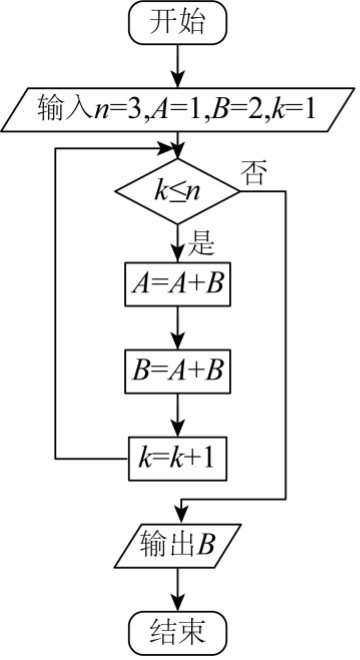
\includegraphics[width=3.4cm]{figures/2023_jia_wen_q6.png}\end{tightcenter}
\fourchoices{$21$}{$34$}{$55$}{$89$}
\item 设$F_1,F_2$为椭圆$C:\dfrac{x^2}{5}+y^2=1$的两个焦点，点$P$在$C$上，若$\vec{PF_1}\cdot\vec{PF_2}=0$，则$|PF_1|\cdot|PF_2|=$
\fourchoices{$1$}{$2$}{$4$}{$5$}
\item 曲线$y=\dfrac{e^x}{x+1}$在点$\left(1,\dfrac e2\right)$处切线方程为
\twochoices{$y=\dfrac e4x$}{$y=\dfrac e2x$}{$y=\dfrac e4x+\dfrac e4$}{$y=\dfrac e2x+\dfrac{3e}4$}
\item 已知双曲线$\dfrac{x^2}{a^2}-\dfrac{y^2}{b^2}=1(a>0,b>0)$的离心率为$\sqrt5$，其中一条渐近线与圆$(x-2)^2+(y-3)^2=1$交于$A,B$两点，则$|AB|=$
\fourchoices{\tallchoice{$\dfrac{\sqrt5}{5}$}}{\tallchoice{$\dfrac{2\sqrt5}{5}$}}{\tallchoice{$\dfrac{3\sqrt5}{5}$}}{\tallchoice{$\dfrac{4\sqrt5}{5}$}}
\item 在三棱锥$P-ABC$中，$\triangle ABC$是边长为$2$的等边三角形，$PA=PB=2$，$PC=\sqrt6$，则该棱锥的体积为
\fourchoices{$1$}{$\sqrt3$}{$2$}{$3$}
\item 已知函数$f(x)=e^{-(x-1)^2}$. 记$a=f\left(\dfrac{\sqrt2}{2}\right)$，$b=f\left(\dfrac{\sqrt3}{2}\right)$，$c=f\left(\dfrac{\sqrt6}{2}\right)$，则
\fourchoices{$b>c>a$}{$b>a>c$}{$c>b>a$}{$c>a>b$}
\item 函数$y=f(x)$的图象由$y=\cos\left(2x+\dfrac\pi6\right)$的图象向左平移$\dfrac\pi6$个单位长度得到，则$y=f(x)$的图象与直线$y=\dfrac12x-\dfrac12$的交点个数为
\fourchoices{$1$}{$2$}{$3$}{$4$}
\end{examquestions}

\examsection{二、填空题：本题共4小题，每小题5分，共20分. }
\begin{examquestions}[start=13]
\item 记$S_n$为等比数列$\{a_n\}$前$n$项和. 若$8S_6=7S_3$，则$\{a_n\}$的公比为\blank. 
\item 若$f(x)=(x-1)^2+ax+\sin\left(x+\dfrac\pi2\right)$为偶函数，则$a=$\blank. 
\item 若$x,y$满足约束条件\linsys{3x-2y\leq3,\\-2x+3y\leq3,\\x+y\geq1}，则$z=3x+2y$的最大值为\blank. 
\item 在正方体$ABCD-A_1B_1C_1D_1$中，$AB=4$，$O$为$AC_1$的中点，若该正方体的棱与球$O$的球面有公共点，则球$O$的半径的取值范围是\blank. 
\end{examquestions}

\examsection{三、解答题：本题共5小题，共60分. 解答应写出文字说明、证明过程或演算步骤. }
\begin{examanswers}[start=17]
\item (12分)

记$\triangle ABC$的内角$A,B,C$的对边分别为$a,b,c$，已知$\dfrac{b^2+c^2-a^2}{\cos A}=2$. 

（1）求$bc$；

（2）若$\dfrac{a\cos B-b\cos A}{a\cos B+b\cos A}\cdot\dfrac bc=1$，求$\triangle ABC$面积. 

\item (12分)

如图，在三棱柱$ABC-A_1B_1C_1$中，$A_1C\perp$平面$ABC$，$\angle ACB=90^\circ$. 

\noindent\begin{minipage}[t]{0.64\linewidth}
（1）证明：平面$ACC_1A_1\perp$平面$BB_1C_1C$；

（2）设$AB=A_1B$，$AA_1=2$，求四棱锥$A_1-BB_1C_1C$的高. 
\end{minipage}\hfill
\begin{minipage}[t]{0.30\linewidth}
\vspace{-0.5em}
\centering
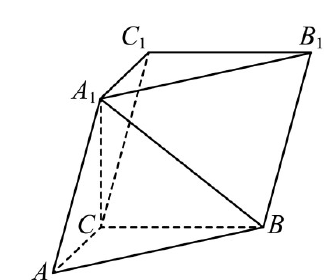
\includegraphics[width=\linewidth]{figures/2023_jia_wen_q18.png}
\end{minipage}

\item(12分)

一项试验旨在研究臭氧效应，试验方案如下：选$40$只小白鼠，随机地将其中$20$只分配到试验组，另外$20$只分配到对照组，试验组的小白鼠饲养在高浓度臭氧环境，对照组的小白鼠饲养在正常环境，一段时间后统计每只小白鼠体重的增加量（单位：g）. 试验结果如下：

对照组的小白鼠体重的增加量从小到大排序为
\begin{center}
    15.2 18.8 20.2 21.3 22.5 23.2 25.8 26.5 27.5 30.1

    32.6 34.3 34.8 35.6 35.6 35.8 36.2 37.3 40.5 43.2
\end{center}

试验组的小白鼠体重的增加量从小到大排序为

\begin{center}

7.8 9.2 11.4 12.4 13.2 15.5 16.5 18.0 18.8 19.2

19.8 20.2 21.6 22.8 23.6 23.9 25.1 28.2 32.3 36.5
\end{center}

（1）计算试验组的样本平均数；

（2）（i）求$40$只小白鼠体重的增加量的中位数$m$，再分别统计两样本中小于$m$与不小于$m$的数据的个数，完成如下列联表：
\begin{tightcenter}\begin{tabular}{|c|c|c|}\hline & $<m$ & $\geq m$ \\\hline 对照组&&\\\hline 试验组&&\\\hline\end{tabular}\end{tightcenter}
（ii）根据（i）中的列联表，能否有$95\%$的把握认为小白鼠在高浓度臭氧环境中与在正常环境中体重的增加量有差异？

附：$K^2=\dfrac{n(ad-bc)^2}{(a+b)(c+d)(a+c)(b+d)}$，
\begin{tightcenter}\begin{tabular}{|c|c|c|c|}\hline $P(K^2\geq k)$&$0.100$&$0.050$&$0.010$\\\hline $k$&$2.706$&$3.841$&$6.635$\\\hline\end{tabular}\end{tightcenter}

\item(12分)

已知函数$f(x)=ax-\dfrac{\sin x}{\cos^2x}$，$x\in\left(0,\dfrac\pi2\right)$. 

（1）当$a=1$时，讨论$f(x)$的单调性；

（2）若$f(x)+\sin x<0$，求$a$的取值范围. 

\item(12分)

已知直线$x-2y+1=0$与抛物线$C:y^2=2px(p>0)$交于$A,B$两点，$|AB|=4\sqrt{15}$. 

（1）求$p$；

（2）设$F$为$C$的焦点，$M,N$为$C$上两点，且$\vec{FM}\cdot\vec{FN}=0$，求$\triangle MFN$面积的最小值. 
\end{examanswers}
\newpage
\examsection{四、选做题：共10分. 请考生在第22、23题中任选一题作答. }
\begin{examanswers}[start=22]
\item(10分)

已知点$P(2,1)$，直线$l:$\linsys{x=2+t\cos\alpha,\\y=1+t\sin\alpha}（$t$为参数），$\alpha$为$l$的倾斜角，$l$与$x$轴正半轴、$y$轴正半轴分别交于$A,B$，且$|PA|\cdot|PB|=4$. 

（1）求$\alpha$；

（2）以坐标原点为极点，$x$轴正半轴为极轴建立极坐标系，求$l$的极坐标方程. 

\item(10分) 

已知$f(x)=2|x-a|-a$，$a>0$. 

（1）求不等式$f(x)<x$的解集；

（2）若曲线$y=f(x)$与$x$轴所围成的图形的面积为$2$，求$a$. 
\end{examanswers}

\end{document}
